\documentclass[11pt]{article}
\usepackage[T1]{fontenc} % Use T1 font encoding
\usepackage[utf8]{inputenc} % Ensure UTF-8 encoding
\usepackage[polish]{babel} % Enable Polish language support
\usepackage{amsmath}
\usepackage{graphicx}
\usepackage{booktabs}
\usepackage{float}
\usepackage[margin=2.5cm]{geometry}
\usepackage{siunitx}
\usepackage{titlesec}
\titlespacing*{\subsection}{0pt}{*0.5}{*0.5} % Adjusts spacing before and after subsections
\usepackage{caption}
\usepackage{lmodern}
\usepackage{placeins} % For FloatBarrier
\usepackage{hyperref} % For hyperlinks in the document
\usepackage{threeparttable} % For better table handling
\usepackage{longtable} % For tables spanning multiple pages
\usepackage{fancyhdr} % For headers and footers
\usepackage{array} % For better table formatting
\usepackage{xcolor} % For colors

\title{Generator RC}
\date{}

\begin{document}

% --------------------------- STRONA TYTUŁOWA --------------------------
\thispagestyle{empty} % Remove page number from title page

\begin{center}
    {\Large\textbf{UNIWERSYTET RADOMSKI}} \\
    \textit{im. Kazimierza Pułaskiego w Radomiu} \\
    \vspace{0.3cm}
    {\large\textbf{LABORATORIUM PODSTAW ELEKTRONIKI}} \\
\end{center}

\vspace{1.5cm}

% Main information box
\begin{center}
\fbox{\begin{minipage}{0.9\textwidth}
\centering
\vspace{0.5cm}
{\Large\textbf{SPRAWOZDANIE Z ĆWICZENIA}} \\
\vspace{0.8cm}
{\LARGE\textbf{Generator RC}} \\
\vspace{0.5cm}
\end{minipage}}
\end{center}

\vspace{1.5cm}

% Information table
\begin{center}
\begin{tabular}{|>{\bfseries}p{4cm}|p{6cm}|}
\hline
Wydział: & WTEiI \\
\hline
Kierunek: & Informatyka \\
\hline
Rok Akademicki: & 2024/2025 \\
\hline
Semestr: & II \\
\hline
Grupa: & 3 \\
\hline
Zespół: & 2 \\
\hline
Wykonujący: & Jakub Oleszczuk \\
& Mateusz Ofiara \\
& Mikołaj Majewski \\
& Onolbataar Tumentur \\
\hline
Ocena: &  \\
\hline
\end{tabular}
\end{center}

\vspace{2cm}

% --------------------------- TREŚĆ SPRAWOZDANIA --------------------------
\subsection*{Cel ćwiczenia}
Celem ćwiczenia było zbadanie działania generatora RC w różnych konfiguracjach oraz analiza wpływu elementów pasywnych na charakterystykę układu.
\subsection*{Wprowadzenie teoretyczne}
Generator RC jest układem elektronicznym, który wykorzystuje rezystory i kondensatory do generowania sygnałów o określonej częstotliwości. W tym ćwiczeniu badaliśmy działanie przesuwania fazy w układzie RC,
 co jest kluczowe dla wielu zastosowań w elektronice, takich jak filtry, oscylatory czy modulatory.
\subsection*{Opis stanowiska pomiarowego}
Stanowisko pomiarowe składało się z generatora sygnału, oscyloskopu oraz przesuwacza Robinsona. Generator sygnału był używany do dostarczania sygnału wejściowego do układu RC, 
a oscyloskop służył do obserwacji i analizy sygnałów wyjściowych. Przesuwacz Robinsona umożliwiał pomiar przesunięcia fazy między sygnałem wejściowym a wyjściowym.
\clearpage
\section*{Wyniki pomiarów}
\begin{table}[!ht]
    \caption{Wyniki pomiarów dla Przesuwnika Robinsona}
    \centering
    \begin{tabular}{|l|l|l|l|l|}
    \hline
        f & U1 & U2 & Bu & FiB \\ \hline
        100 & 1 & 0.152 & 0.152 & 65.6 \\ \hline
        300 & 1 & 0.296 & 0.296 & 30.3 \\ \hline
        630 & 1 & 0.36 & 0.36 & 1.5 \\ \hline
        900 & 1 & 0.348 & 0.348 & -12.2 \\ \hline
        1200 & 1 & 0.344 & 0.344 & -23.4 \\ \hline
        1600 & 1 & 0.314 & 0.314 & -34.6 \\ \hline
        2500 & 1 & 0.23 & 0.23 & -51 \\ \hline
        3200 & 1 & 0.192 & 0.192 & -59.3 \\ \hline
    \end{tabular}
\end{table}
\begin{figure}
    \centering
    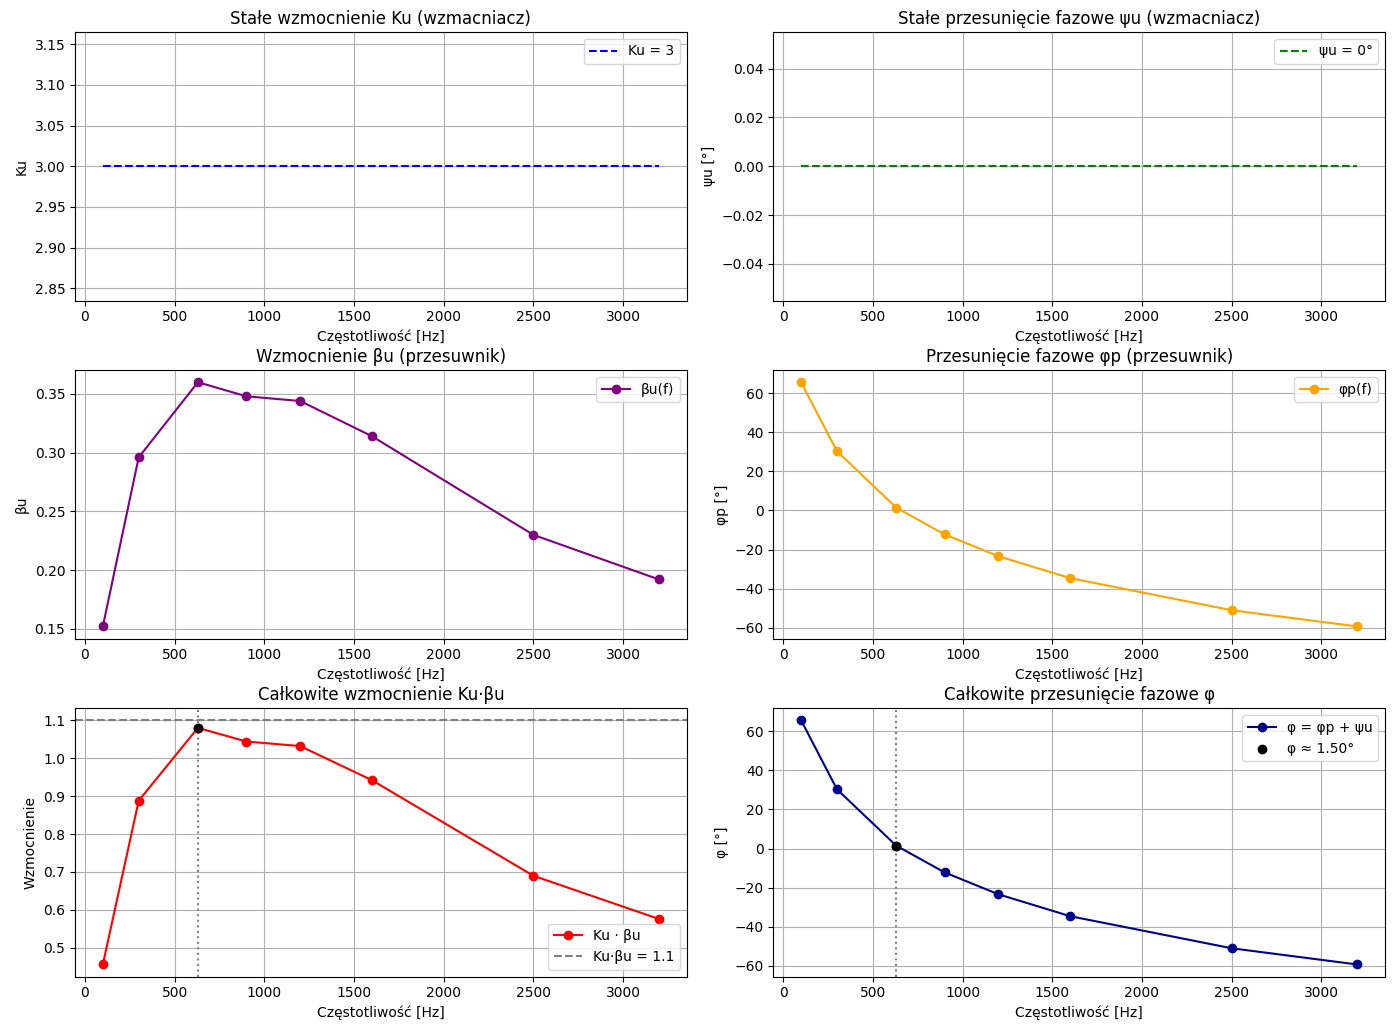
\includegraphics[width=0.8\textwidth]{Generator.png}
    \label{fig:robinson}
\end{figure}

\FloatBarrier % Ensures that all floats are processed before continuing

\subsection*{Analiza wyników}
Wyniki pomiarów pokazują, że przesunięcie fazy między sygnałem wejściowym a wyjściowym zmienia się w zależności od częstotliwości. Dla niskich częstotliwości przesunięcie fazy jest większe,
natomiast dla wyższych częstotliwości maleje. To potwierdza teoretyczne założenia dotyczące działania układu RC, gdzie przesunięcie fazy jest funkcją częstotliwości sygnału.
Potencjalnym punktem generacji to 630 Hz, gdzie przesunięcie fazy wynosi 1.5 stopnia. Wartości przesunięcia fazy dla innych częstotliwości również są zgodne z oczekiwaniami teoretycznymi.
\subsection*{Podsumowanie}
W ćwiczeniu zbadaliśmy działanie generatora RC oraz przesuwacza Robinsona. Wyniki pomiarów potwierdziły teoretyczne założenia dotyczące przesunięcia fazy w układzie RC.
Zrozumieliśmy, jak elementy pasywne wpływają na charakterystykę układu oraz jak można wykorzystać te właściwości w praktycznych zastosowaniach elektronicznych.
\subsection*{Wnioski}
Z przeprowadzonego ćwiczenia wynika, że generator RC jest skutecznym narzędziem do generowania sygnałów o określonej częstotliwości. 
Przesunięcie fazy jest istotnym parametrem, który należy uwzględnić w projektowaniu układów elektronicznych.

\end{document}
